%%%%%%%%%%%%%%%%%%%%%%%%%%%%%%%%%%%%%%%%%
% Arsclassica Article
% LaTeX Template
% Version 1.1 (10/6/14)
%
% This template has been downloaded from:
% http://www.LaTeXTemplates.com
%
% Original author:
% Lorenzo Pantieri (http://www.lorenzopantieri.net) with extensive modifications by:
% Vel (vel@latextemplates.com)
%
% License:
% CC BY-NC-SA 3.0 (http://creativecommons.org/licenses/by-nc-sa/3.0/)
%
%%%%%%%%%%%%%%%%%%%%%%%%%%%%%%%%%%%%%%%%%

%----------------------------------------------------------------------------------------
%	PACKAGES AND OTHER DOCUMENT CONFIGURATIONS
%----------------------------------------------------------------------------------------

\documentclass[
10pt, % Main document font size
a4paper, % Paper type, use 'letterpaper' for US Letter paper
oneside, % One page layout (no page indentation)
%twoside, % Two page layout (page indentation for binding and different headers)
headinclude,footinclude, % Extra spacing for the header and footer
BCOR5mm, % Binding correction
]{scrartcl}

%%%%%%%%%%%%%%%%%%%%%%%%%%%%%%%%%%%%%%%%%
% Arsclassica Article
% Structure Specification File
%
% This file has been downloaded from:
% http://www.LaTeXTemplates.com
%
% Original author:
% Lorenzo Pantieri (http://www.lorenzopantieri.net) with extensive modifications by:
% Vel (vel@latextemplates.com)
%
% License:
% CC BY-NC-SA 3.0 (http://creativecommons.org/licenses/by-nc-sa/3.0/)
%
%%%%%%%%%%%%%%%%%%%%%%%%%%%%%%%%%%%%%%%%%

%----------------------------------------------------------------------------------------
%	REQUIRED PACKAGES
%----------------------------------------------------------------------------------------

\usepackage[
nochapters, % Turn off chapters since this is an article        
beramono, % Use the Bera Mono font for monospaced text (\texttt)
eulermath,% Use the Euler font for mathematics
pdfspacing, % Makes use of pdftex’ letter spacing capabilities via the microtype package
dottedtoc % Dotted lines leading to the page numbers in the table of contents
]{classicthesis} % The layout is based on the Classic Thesis style

\usepackage{arsclassica} % Modifies the Classic Thesis package

\usepackage[T1]{fontenc} % Use 8-bit encoding that has 256 glyphs

\usepackage[utf8]{inputenc} % Required for including letters with accents

\usepackage{graphicx} % Required for including images
\graphicspath{{Figures/}} % Set the default folder for images

\usepackage{enumitem} % Required for manipulating the whitespace between and within lists

\usepackage{lipsum} % Used for inserting dummy 'Lorem ipsum' text into the template

\usepackage{subfig} % Required for creating figures with multiple parts (subfigures)

\usepackage{amsmath,amssymb,amsthm} % For including math equations, theorems, symbols, etc

\usepackage{varioref} % More descriptive referencing

%----------------------------------------------------------------------------------------
%	THEOREM STYLES
%---------------------------------------------------------------------------------------

\theoremstyle{definition} % Define theorem styles here based on the definition style (used for definitions and examples)
\newtheorem{definition}{Definition}

\theoremstyle{plain} % Define theorem styles here based on the plain style (used for theorems, lemmas, propositions)
\newtheorem{theorem}{Theorem}

\theoremstyle{remark} % Define theorem styles here based on the remark style (used for remarks and notes)

%----------------------------------------------------------------------------------------
%	HYPERLINKS
%---------------------------------------------------------------------------------------

\hypersetup{
%draft, % Uncomment to remove all links (useful for printing in black and white)
colorlinks=true, breaklinks=true, bookmarks=true,bookmarksnumbered,
urlcolor=webbrown, linkcolor=RoyalBlue, citecolor=webgreen, % Link colors
pdftitle={}, % PDF title
pdfauthor={\textcopyright}, % PDF Author
pdfsubject={}, % PDF Subject
pdfkeywords={}, % PDF Keywords
pdfcreator={pdfLaTeX}, % PDF Creator
pdfproducer={LaTeX with hyperref and ClassicThesis} % PDF producer
} % Include the structure.tex file which specified the document structure and layout

\hyphenation{Fortran hy-phen-ation} % Specify custom hyphenation points in words with dashes where you would like hyphenation to occur, or alternatively, don't put any dashes in a word to stop hyphenation altogether

%----------------------------------------------------------------------------------------
%	TITLE AND AUTHOR(S)
%----------------------------------------------------------------------------------------

\title{\normalfont\spacedallcaps{Algebra for Security Documentation}} % The article title

\author{\spacedlowsmallcaps{Jeroen Ubbink \& René Wouters}} % The article author(s) - author affiliations need to be specified in the AUTHOR AFFILIATIONS block

\date{\today} % An optional date to appear under the author(s)

%----------------------------------------------------------------------------------------

\begin{document}

%----------------------------------------------------------------------------------------
%	HEADERS
%----------------------------------------------------------------------------------------

\renewcommand{\sectionmark}[1]{\markright{\spacedlowsmallcaps{#1}}} % The header for all pages (oneside) or for even pages (twoside)
%\renewcommand{\subsectionmark}[1]{\markright{\thesubsection~#1}} % Uncomment when using the twoside option - this modifies the header on odd pages
\lehead{\mbox{\llap{\small\thepage\kern1em\color{halfgray} \vline}\color{halfgray}\hspace{0.5em}\rightmark\hfil}} % The header style

\pagestyle{scrheadings} % Enable the headers specified in this block

%----------------------------------------------------------------------------------------
%	TABLE OF CONTENTS & LISTS OF FIGURES AND TABLES
%----------------------------------------------------------------------------------------

\maketitle % Print the title/author/date block

\setcounter{tocdepth}{2} % Set the depth of the table of contents to show sections and subsections only

\tableofcontents % Print the table of contents

\listoffigures % Print the list of figures

% \listoftables % Print the list of tables

%----------------------------------------------------------------------------------------
%	ABSTRACT
%----------------------------------------------------------------------------------------


%----------------------------------------------------------------------------------------
%	AUTHOR AFFILIATIONS
%----------------------------------------------------------------------------------------

%{\let\thefootnote\relax\footnotetext{*}}

%{\let\thefootnote\relax\footnotetext{}}}

%----------------------------------------------------------------------------------------

\newpage % Start the article content on the second page, remove this if you have a longer abstract that goes onto the second page

%----------------------------------------------------------------------------------------
%	INTRODUCTION
%----------------------------------------------------------------------------------------

\section{Introduction}

This is the report accompanying the code submission for 2WF70, Algebra for Security. This document will serve as a user guide and feature documentation of the Polynomial calculator program, outlining the the operations the program is capable of performing, and how it does so.

 
%----------------------------------------------------------------------------------------
%	METHODS
%----------------------------------------------------------------------------------------

\section{Methods}
\subsection{Input Requirements}
The requirements for the program were as follows:
\begin{itemize}


\item Polynomial Objects
	\begin{enumerate}[noitemsep]
	\item Input two polynomials with integer coefficients modulo a prime, with output of the sum, returning the sum, product, and difference of the two entered polynomials.
	\item Input a polynomial with integer coefficients modulo a prime, and a scalar coefficient, returning the polynomial after being scaled.
	\item Input two polynomials with integer coefficients modulo a prime, return the quotient and remainder through long division.
	\item For coefficients modulo a prime, implement the (Extended) Euclidean Algorithm, returning 
	\item For input of three polynomials, return true if the first two polynomials are equal to each other modulo the third polynomial.
	\end{enumerate}

\item Finite Field Objects
	\begin{enumerate}[noitemsep]
	\item Upon input of a prime number and an irreducible polynomial $q(X)$, return the addition and multiplication table of $\mathbb{Z}/p\mathbb{Z}[X]/(q(X))$.
	\item Upon input of two field elements $a$ and $b$, return the sum, the product, and the quotient $ab^{-1}$ in a field.
	\item Upon input of a field and field element, return the primitivity of the element.
	\item Upon input of a field, return the primitive elements of the field.
	\item Upon input of a polynomial modulo a prime, test the irreducibility, and produce the irreducible polynomials of the prescribed degree. 
	\end{enumerate}
\end{itemize}

Our implementation currently implements all of the Polynomial object methods, and none of the Finite Field Object methods.
%------------------------------------------------

\subsection{Overview of Program}

Our program is split into three classes, the main class, which parses input. The polynomial class, which defines the polynomial class of objects, and the finite field class, which defined the finite field class of objects.

\paragraph{Parser}
Our parser class has a number of methods, but generally works through parsing the input stream, and depending on the input selectors, selects one of the ten cases, and then calls a method in order to parse the remainder of the input stream to convert the text input into polynomial objects if necessary. It also parses the input stream to integers.//

The input strings required for each operation are as follows:\\
\textbf{Polynomial objects:}
\begin{enumerate}[noitemsep]
\item poly basic polynomial1 polynomial2 prime, where the first two words are strings, the next two strings are polynomial objects, and the prime is an integer.

\item poly scalar polynomial1 coefficient prime, where the first two words are strings, the next string is a polynomial object, and the next two strings are integers.

\item poly division polynomial1 polynomial2 prime, where the first two words are strings, the next two strings are polynomial objects, and the final string is an integer.

\item poly GCD polynomial1 polynomial2 prime, where the first two words are strings, the next two strings are polynomial objects, and the final string is an integer.

\item poly polymod polynomial1 polynomial2 polynomial3, where the first two words are strings, and the three polynomial objects are the polynomials that you would like to compare to each other.
\end{enumerate}

It is important to note here that strings must be entered \textit{exactly} as above (including capitals), meaning the first two words in the input. The polynomials must always have a term included, with an example as follows: $-2X^-3 -1X^0$. As seen, it is allowed to have negative coefficients and exponents. Finally, for input of all integers, negatives are allowed.\\

Finite Field inputs have not currently been implemented, and thus return an error message if the first string is FF, which has been chosen as the selector for that set of inputs.\\


\paragraph{Polynomial}
The Polynomial class defines the object used to hold a polynomial, which is done through a HashMap, which stores the set of exponents as an index, which maps to the coefficients. It also has an integer value $modulus$, which holds the modulo for the polynomial, which if uninitialized is the maximum value $-1$ of an integer in java. The coefficients have mod $modulus$ applied to them after every operation that changes their value.\\

This class also has all of the methods to perform operations on polynomial objects, with standard get and set methods for the "terms" Hashmap and the "modulus" integers.\\

The methods in order to do Long Division(Algorithm 1.2.6), Greatest Common Divisor (Algorithm 1.2.10), and extended GCD(Algorithm 1.2.11) operations are from the book, modified to use for each loops to iterate through the HashMaps in order to get the values to perform the computations.\\

The methods in order to do addition, subtraction, and multiplication were done through for each loops (nested for each loops for multiplication) to iterate through the terms in order to do the operations. Currently, the implementation does not remove terms if the coefficient is zero.\\

\paragraph{Finite Fields}
Currently does not do anything.

%------------------------------------------------
\subsection{Proof of Function}
% TODO
\paragraph{Basic Methods}
poly basic polynomial1 polynomial2 prime, where the first two words are strings, the next two strings are polynomial objects, and the prime is an integer.

\paragraph{Scalar Multiplication}
poly scalar polynomial1 coefficient prime, where the first two words are strings, the next string is a polynomial object, and the next two strings are integers.

\paragraph{Long Division}
poly division polynomial1 polynomial2 prime, where the first two words are strings, the next two strings are polynomial objects, and the final string is an integer.

\paragraph{(Extended) Euclid's Algorithm}
poly GCD polynomial1 polynomial2 prime, where the first two words are strings, the next two strings are polynomial objects, and the final string is an integer.

\paragraph{Two Polynomials Modulo Another}
poly polymod polynomial1 polynomial2 polynomial3, where the first two words are strings, and the three polynomial objects are the polynomials that you would like to compare to each other.


\iffalse
%----------------------------------------------------------------------------------------
%	RESULTS AND DISCUSSION
%----------------------------------------------------------------------------------------

\section{Results and Discussion}

\lipsum[10] % Dummy text

%------------------------------------------------

\subsection{Subsection}

\lipsum[11] % Dummy text

\subsubsection{Subsubsection}

\lipsum[12] % Dummy text

\begin{description}
\item[Word] Definition
\item[Concept] Explanation
\item[Idea] Text
\end{description}

\lipsum[12] % Dummy text

\begin{itemize}[noitemsep] % [noitemsep] removes whitespace between the items for a compact look
\item First item in a list
\item Second item in a list
\item Third item in a list
\end{itemize}

\subsubsection{Table}

\lipsum[13] % Dummy text

\begin{table}[hbt]
\caption{Table of Grades}
\centering
\begin{tabular}{llr}
\toprule
\multicolumn{2}{c}{Name} \\
\cmidrule(r){1-2}
First name & Last Name & Grade \\
\midrule
John & Doe & $7.5$ \\
Richard & Miles & $2$ \\
\bottomrule
\end{tabular}
\label{tab:label}
\end{table}

Reference to Table~\vref{tab:label}. % The \vref command specifies the location of the reference

%------------------------------------------------

\subsection{Figure Composed of Subfigures}

Reference the figure composed of multiple subfigures as Figure~\vref{fig:esempio}. Reference one of the subfigures as Figure~\vref{fig:ipsum}. % The \vref command specifies the location of the reference

\lipsum[15-18] % Dummy text

%\begin{figure}[tb]
%\centering
%\subfloat[A city market.]{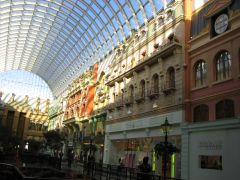
\includegraphics[width=.45\columnwidth]{Lorem}} \quad
%\subfloat[Forest landscape.]{
\includegraphics[width=.45\columnwidth]{Ipsum}%\label{fig:ipsum}} \\
%\subfloat[Mountain landscape.]{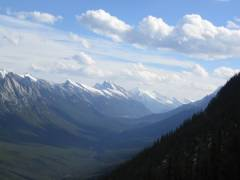
\includegraphics[width=.45\columnwidth]{Dolor}} \quad
%\subfloat[A tile decoration.]{
\includegraphics[width=.45\columnwidth]{Sit}}
%\caption[A number of pictures.]{A number of pictures with no common theme.} % The %text in the square bracket is the caption for the list of figures while the text in %the curly brackets is the figure caption
%\label{fig:esempio}
%\end{figure}
\fi
%----------------------------------------------------------------------------------------
%	BIBLIOGRAPHY
%----------------------------------------------------------------------------------------

\renewcommand{\refname}{\spacedlowsmallcaps{References}} % For modifying the bibliography heading

\bibliographystyle{unsrt}

\bibliography{sample.bib} % The file containing the bibliography

%----------------------------------------------------------------------------------------

\end{document}